% FD analysis chapter -- using shower reconstruction to distinguish pi0s and electrons?
% Target: 10 pages

\graphicspath{{FarDetectorAnalysis/Figs/}}

%----------------------------------------------------------------------------------------------------------------------------------------------------------------------------
%\chapter{Electron Reconstruction for $\nu_e$ Oscillation Signal at the DUNE Far Detector}\label{chap:FDAnalysis}
\chapter{The $\nu_e$ Oscillation Signal at the DUNE Far Detector}\label{chap:FDAnalysis}

A primary aim of the DUNE experiment, as discussed in Chapter~\ref{chap:DUNE}, is to make precision measurements of the PMNS matrix parameters describing neutrino oscillations by searching for electron neutrino appearance from the predominantly muon neutrino beam (i.e. $\nu_{\mu} \rightarrow \nu_e$ oscillation, described by Equation~\ref{eq:ElectronNeutrinoAppearance}).  This channel is of critical importance for all oscillation-related physics and thus requires very efficient reconstruction and selection.  Methods developed to provide reconstruction of these events were discussed in detail in Chapter~\ref{chap:LArTPCReconstruction} and utilised in this present chapter in the selection of simulated charged-current (CC) $\nu_e$ events ($\nu_e$CC) in the DUNE far detector.

The selection presented in the following sections represents the very first generation analysis for the DUNE experiment and serves primarily to demonstrate the principle of selecting these events in a large LArTPC.\footnote{This work was undertaken with Dominic Brailsford (Lancaster University), who was working on the complementary $\nu_{\mu}$CC selection.}  Initially, the samples and simulation methods utilised in the selection are very briefly discussed in Section~\ref{sec:FDSamples}.  Much work is needed to advance the analysis to comply with DUNE requirements and many improvements may be expected as further developments progress.  It should also be noted the reconstruction discussed in Chapter~\ref{chap:LArTPCReconstruction} is not the only solution and various other techniques, primarily using the Pandora toolkit \cite{Pandora2015}, have been assessed, notably in Section~\ref{sec:FDCut}.  The selection presented in Section~\ref{sec:FDMVA} does utilise the novel reconstruction detailed in this thesis; however, due to significant recent progress, it is likely the selection will continue to explore all reconstructions in LArSoft and take advantage of the continuing developments.  This outlook will be briefly discussed in Section~\ref{sec:FDOutlook}.

%----------------------------------------------------------------------------------------------------------------------------------------------------------------------------
\section{Far Detector Samples}\label{sec:FDSamples}

The selections discussed in this chapter aim to separate $\nu_e$ events from $\nu_{\mu}$ and $\nu_{\tau}$ events.  Samples of 100,000 of each of these particle species were generated within LArSoft for use in the tuning and the running of the analysis.

The neutrinos in the samples were generated as a simulated particle beam, with mostly $\nu_{\mu}$s and a small accidental contamination from other species, before exchanging the flavours to simulate oscillations.  This ensures the correct energy spectrum for all neutrinos arriving at the far detector.  In the case of the $\nu_e$ sample, the muon neutrinos are swapped for electron neutrinos and the beam electron neutrinos for tau neutrinos; in the $\nu_{\tau}$ sample, the muon neutrinos are swapped for tau neutrinos (MIKE take into account the tau threshold or are these NC?) and the beam electron neutrino component for muon neutrinos.  When used, these events are then weighted according to the relevant oscillation probabilities for the specific transitions simulated, determined by the neutrino energy and the current understanding of the mixing parameters (described in Section~\ref{sec:OscillationParameters}).

The events are also scaled to ensure the correct POT (protons-on-target) weighting.  The charged-current events in each sample are de-weighted by the number of events and the neutral-current events are de-weighted by the number of events in all three samples.  The scaling then weights all events to the same POT (here, $1\times10^{21}$ is used).

%----------------------------------------------------------------------------------------------------------------------------------------------------------------------------
\section{Cut-Based Tuning}\label{sec:FDCut}

This section details the early developments of a selection which utilises only Pandora reconstruction and a cut-based approach.  This procedure shows promise at performing as well as the more established multi-variate analysis (MVA) method, discussed in Section~\ref{sec:FDMVA}, but is used here mainly to tune the selection.

As will be discussed in Section~\ref{sec:FDMVA}, the current MVA implementation of the $\nu_e$CC selection contains a mixture of particle-level and event-level variables and requires significant understanding before developments may progress.  The motivation behind considering a simplified selection is to facilitate a careful evaluation of the events, and the analysis utilises a distinct particle identification (PID) system to perform particle level discrimination, separate from the event level classification.  As with the majority of this present chapter, this work is very preliminary and represents the first studies into these areas for the DUNE experiment.

%----------------------------------------------------------------------------------------------------------------------------------------------------------------------------
\subsection{Selection}\label{sec:FDCutSelection}

The elementary cut-based selection utilises Pandora reconstruction for tracks and showers and an MVA approach to PID for each of the reconstructed objects.  This PID framework \cite{GrantPID2016} utilises variables such as (MIKE define variables) ratios of deposited charge, conicalness, average dE/dx and dE/dx ratios to form a hypothesis for each of the particle types muon, electron, proton, photon, pion.  The selection simply selects events which contain candidate electron showers and places a cut on the value of the electron-MVA result to attempt to identify the electrons.  The separation between electrons and photons for the electron-MVA value of the highest energy shower in each event is demonstrated in Figure~\ref{fig:ElectronMVA}.  It is immediately evident that, given the strengths of LArTPC technology to separate these showering particle types, significant progress is required in the next decade.

\begin{figure}
  \centering
  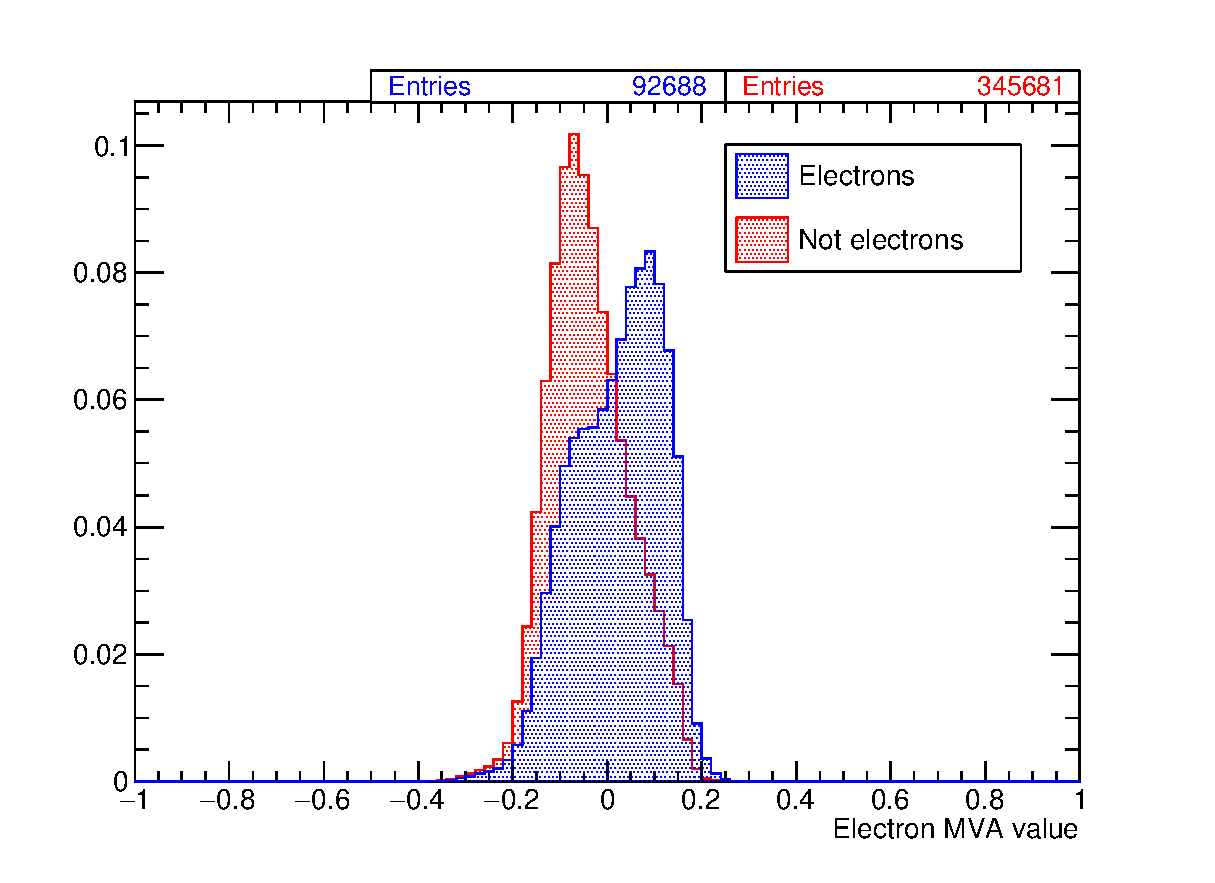
\includegraphics[width=10cm]{ElectronMVA.eps}
  \caption[The output of a multi-variate approach to particle identification when attempting to identify electrons.]{The output of a multi-variate approach to particle identification when attempting to identify electrons.}
  \label{fig:ElectronMVA}
\end{figure}

To tune this cut, and for further tunings discussed in Section~\ref{sec:FDCutFV}, a physics-based approach was taken.  Arguably the most important consequence of this analysis, since the value of $\theta_{13}$ is reasonably well understood, is to search for CP-violation, and so the tuning was designed to maximise its capability for this.  For each electron-MVA value, the $\nu_e$-appearance energy spectrum was determined for the CP-conservation ($\delta_{CP}=0$) and CP-violation ($\delta_{CP}=\pi/2$) hypotheses; maximising the $\chi^2$ between the distributions ensures the greatest discriminating ability of the analysis to discern hints of CP-violation.  This is demonstrated in Figure~\ref{fig:ElectronMVATune}, and a cut value of 0.02 is found to provide the best differentiation.  The events were POT-weighted and the oscillation probabilities were provided extemporaneously by the Prob3++ framework \cite{Prob3++}.

\begin{figure}
  \centering
  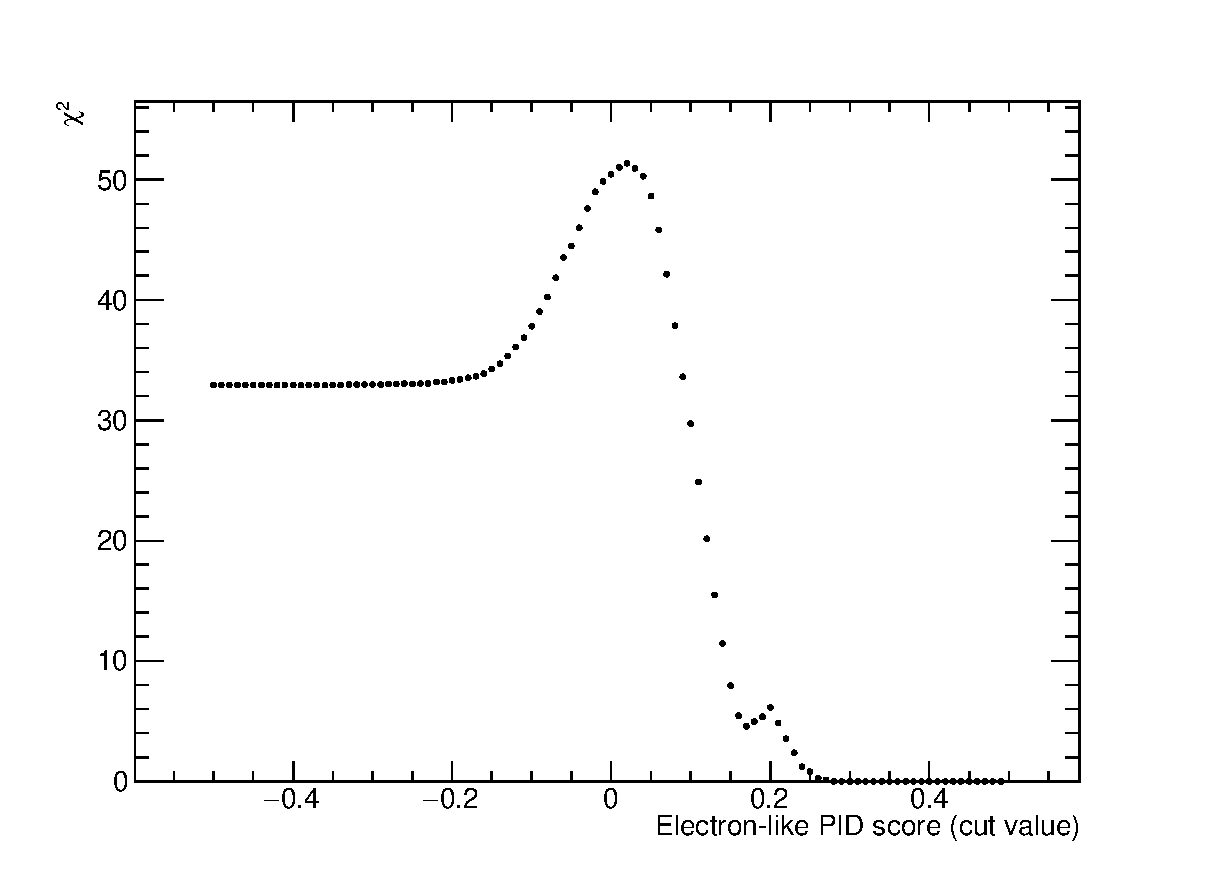
\includegraphics[width=10cm]{ElectronMVATune.eps}
  \caption[The process of tuning the electron cut in the simple cut-based selection by maximising the effect of CP-violation on the oscillation probabilities.]{The process of tuning the electron cut in the simple cut-based selection by maximising the effect of CP-violation on the oscillation probabilities.}
  \label{fig:ElectronMVATune}
\end{figure}

In order to assess the efficacy of the analysis, the commonly used efficiency and purity metrics may be employed.  The efficiency represents how many of the total number of signal events are chosen by the analysis and the purity describes the fraction of the selected events which are indeed signal.  The efficiency and purity of the selection with just this simple cut is demonstrated in Figure~\ref{fig:EffPurCutSelection}.  It is found the selection already looks reasonable, with an overall efficiency of 76\% and purity of 35\%, and, as will be observed and discussed further in Section~\ref{sec:FDMVA}, is competitive with the MVA-based analysis.

\begin{figure}
  \centering
  \begin{subfigure}[t]{0.48\linewidth}
    \centering
    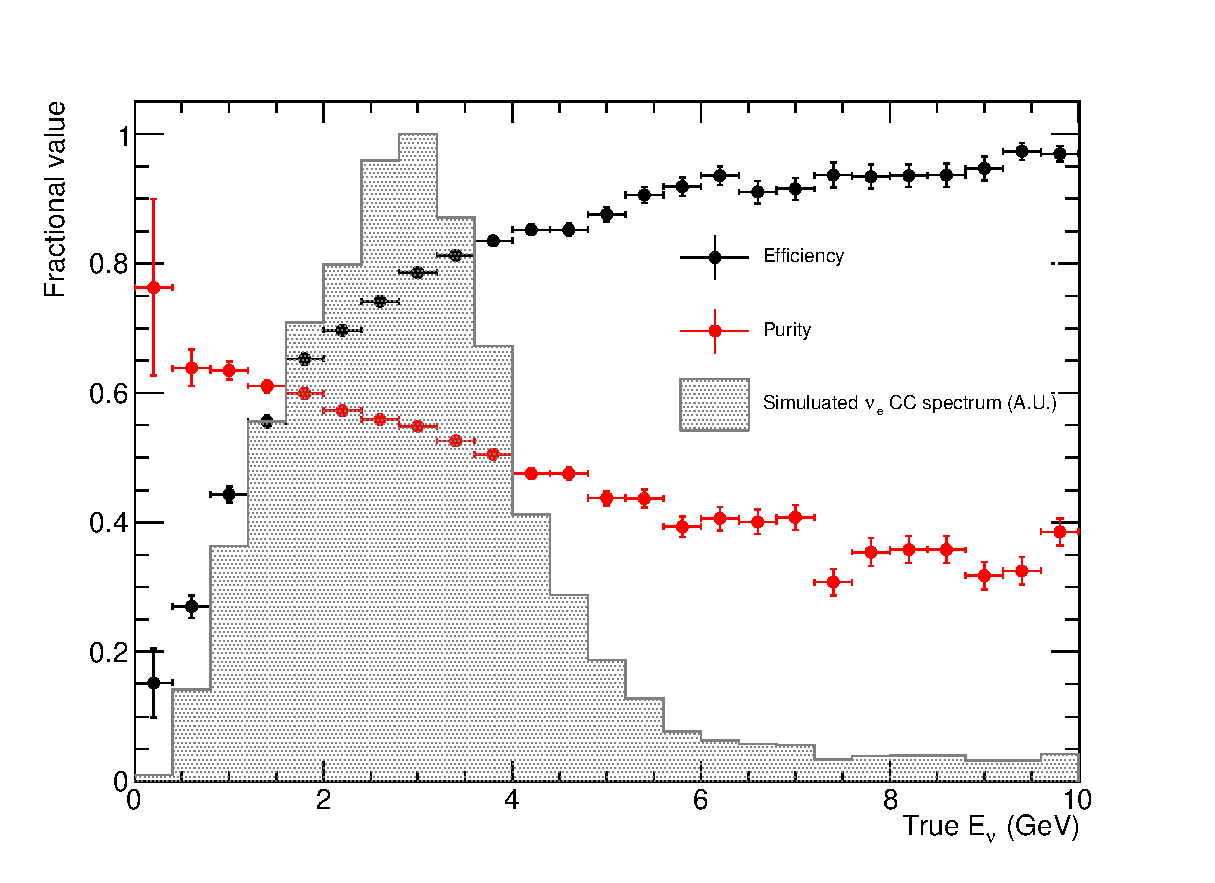
\includegraphics[width=0.98\textwidth]{ENuCutSelection.eps}
    \caption{$E_{\nu}$}
    \label{fig:ENuCutSelection}
  \end{subfigure}
  \hfill
  \begin{subfigure}[t]{0.48\linewidth}
    \centering
    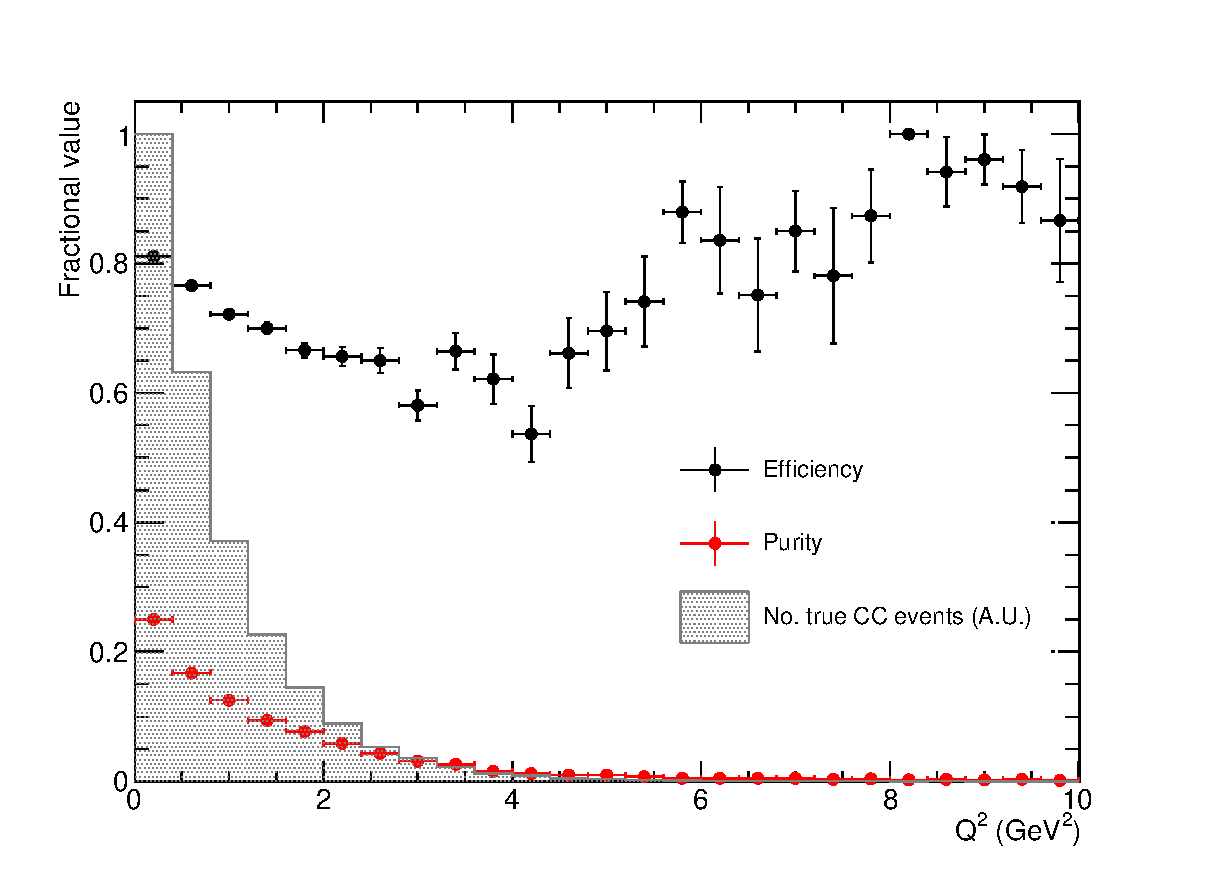
\includegraphics[width=0.98\textwidth]{Q2CutSelection.eps}
    \caption{$Q^2$}
    \label{fig:Q2CutSelection}
  \end{subfigure}
  \vfill
  \begin{subfigure}[t]{0.48\linewidth}
    \centering
    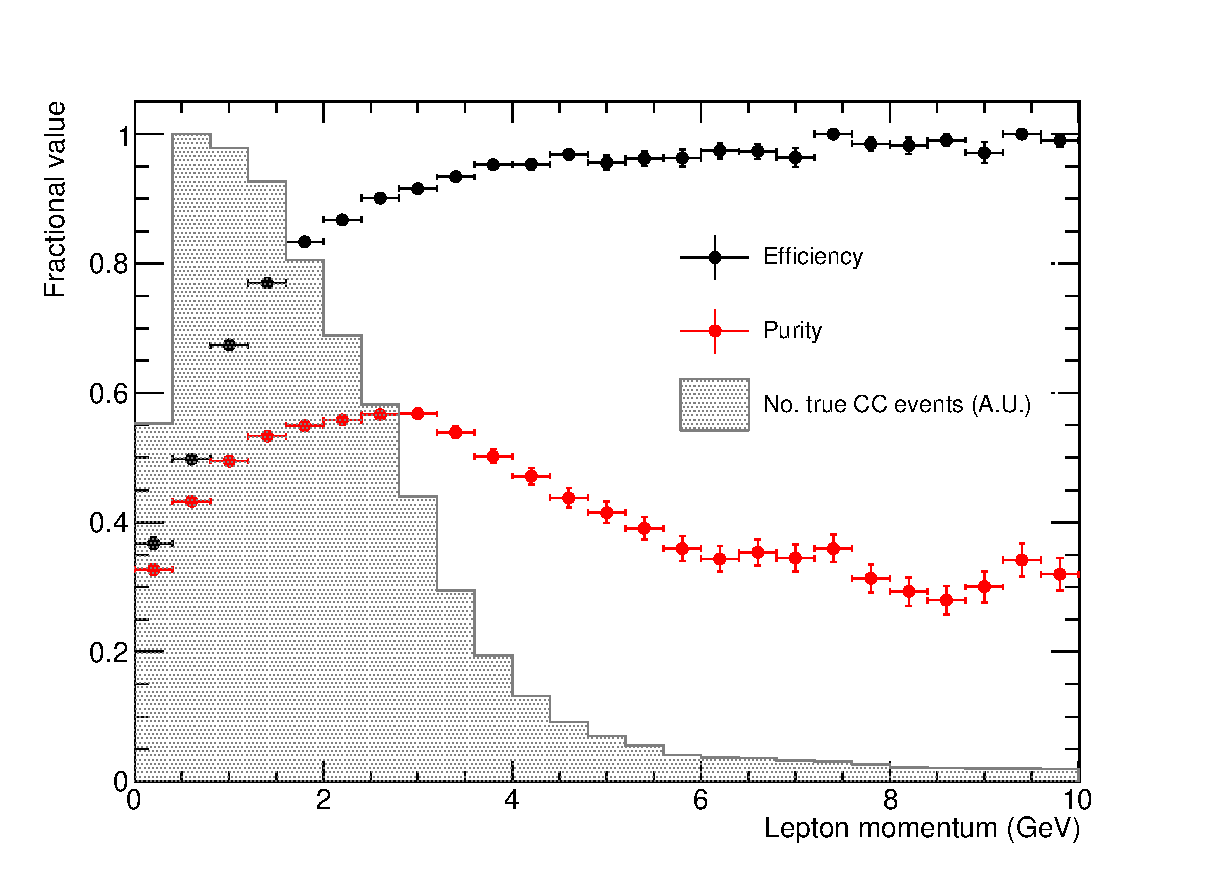
\includegraphics[width=0.98\textwidth]{LeptonMomentumCutSelection.eps}
    \caption{Lepton momentum}
    \label{fig:LeptonMomentumCutSelection}
  \end{subfigure}
  \hfill
  \begin{subfigure}[t]{0.48\linewidth}
    \centering
    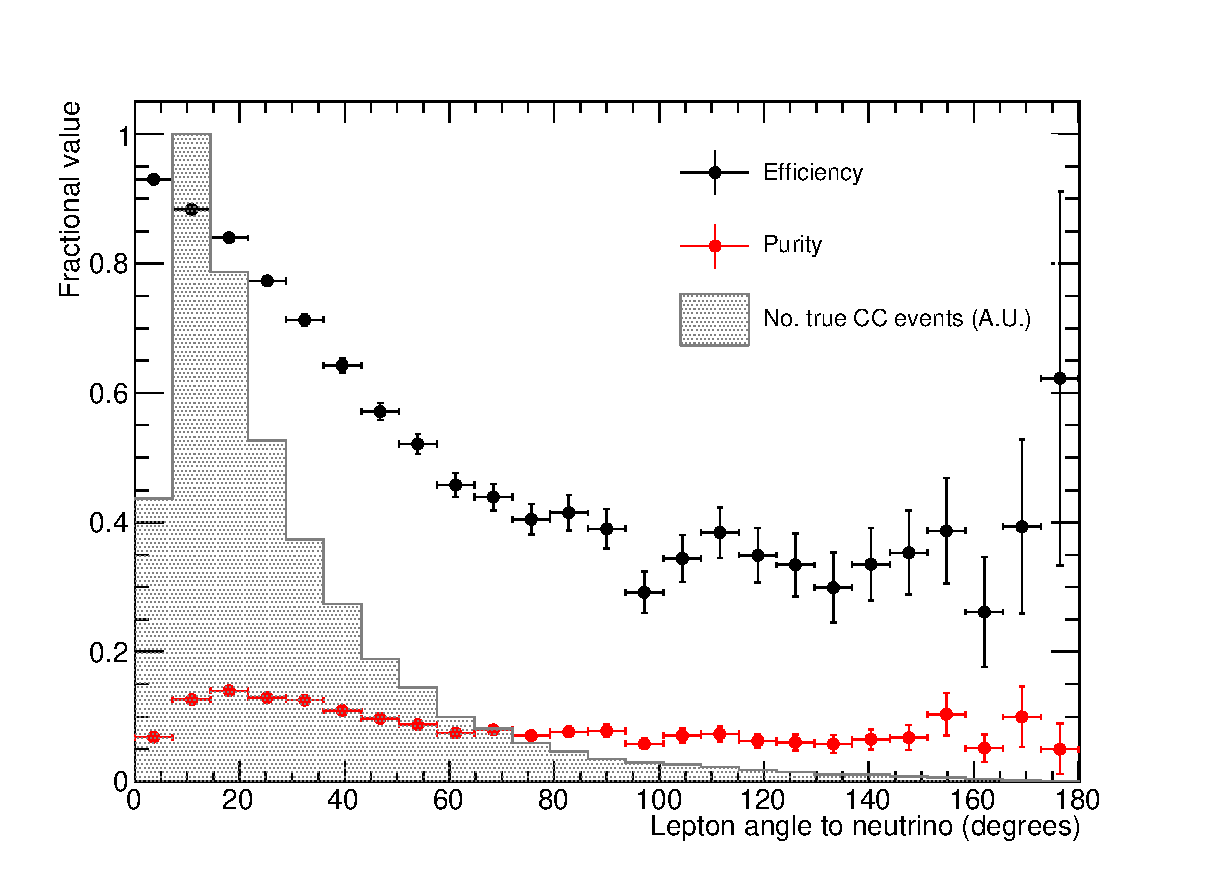
\includegraphics[width=0.98\textwidth]{LeptonAngleCutSelection.eps}
    \caption{Lepton angle}
    \label{fig:LeptonAngleCutSelection}
  \end{subfigure}
  \caption[The efficiency and purity of the $\nu_e$CC Pandora cut-based selection as a function of a number of kinematic variables, after applying the selection.]{The efficiency and purity of the $\nu_e$CC Pandora cut-based selection as a function of a number of kinematic variables, after applying the selection.  The variables are the true neutrino energy (Figure~\ref{fig:ENuCutSelection}), the true momentum transfer, $Q^2$ (Figure~\ref{fig:Q2CutSelection}), the electron momentum (Figure~\ref{fig:LeptonMomentumCutSelection}) and the angle the electron makes to the neutrino beam (Figure~\ref{fig:LeptonAngleCutSelection}).  The plots are filled for each event which passes the cut (highest energy shower PID MVA response $>0.02$).}
  \label{fig:EffPurCutSelection}
\end{figure}

%----------------------------------------------------------------------------------------------------------------------------------------------------------------------------
\subsection{Fiducial Volume Tuning}\label{sec:FDCutFV}

A similar approach to the tuning described in the previous section may be utilised to optimise the fiducial volume (FV) applied in the selection.  This has not previously been performed in the DUNE far detector, with estimations and assumptions applied during the development of the analysis.  The distance of the start point of the electron shower from the walls of the cryostat is considered over a range of energies and oscillation probabilities, as before, and the $\chi^2$ between the distributions for maximum CP-conservation and CP-violation maximised to provide the optimal parameters.

Example plots showing the tuning of the $y$-coordinate are the subject of Figure~\ref{fig:FVTuneY}.  The tuned FD coordinates, along with the cryostat dimensions, are shown in Table~\ref{tab:FV}.  It should again be noted this is a preliminary study and this volume would be expected to change with more advanced simulation and reconstruction.  In particular, a fully inclusive region in the upstream beam direction ($-z$), implied by these results, will include much activity from the rock and will be better tuned when using a more detailed simulation including deeper rock interactions.

\begin{figure}
  \centering
  \begin{subfigure}[t]{0.48\linewidth}
    \centering
    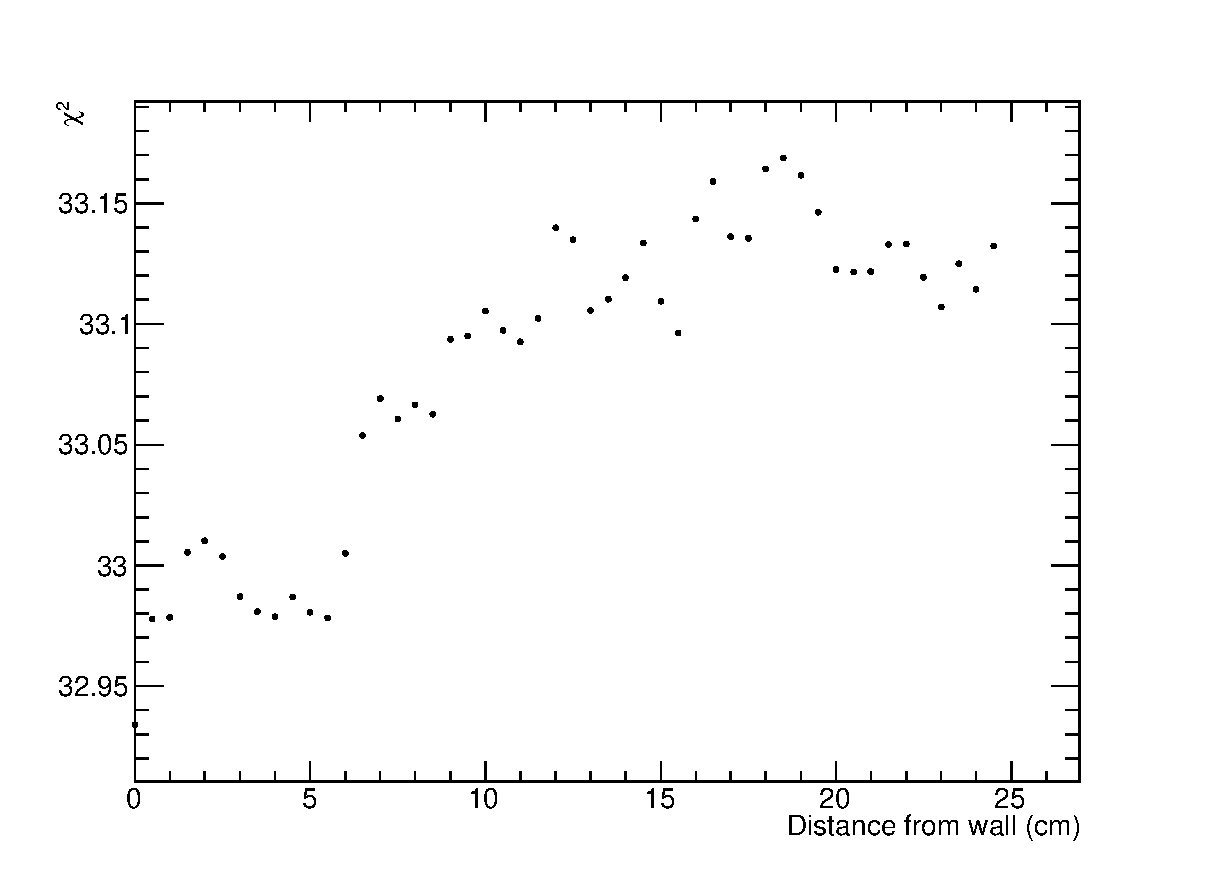
\includegraphics[width=0.98\textwidth]{FVTunePosY.eps}
    \caption{$+y$}
    \label{fig:FVTunePosY}
  \end{subfigure}
  \hfill
  \begin{subfigure}[t]{0.48\linewidth}
    \centering
    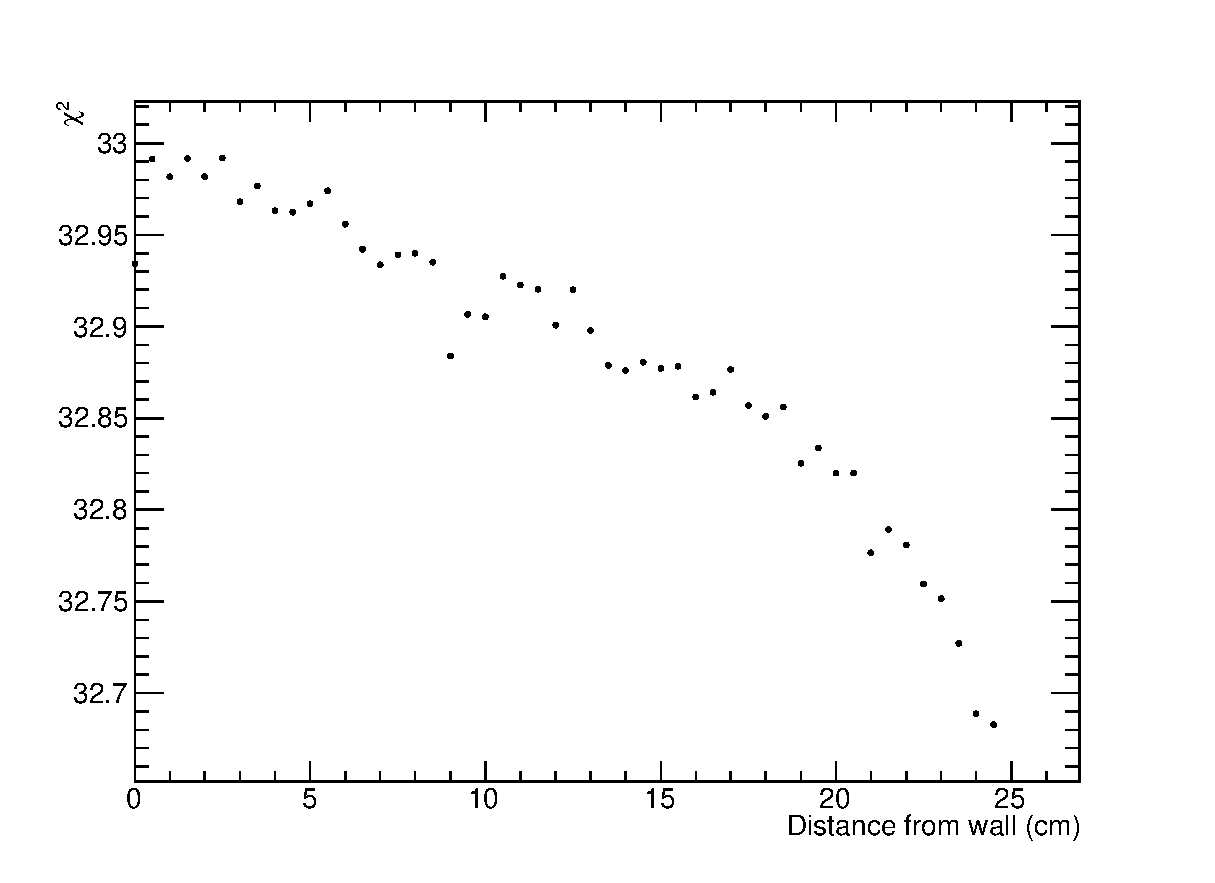
\includegraphics[width=0.98\textwidth]{FVTuneNegY.eps}
    \caption{$-y$}
    \label{fig:FVTuneNegY}
  \end{subfigure}
  \caption[Tuning the DUNE far detector fiducial volume, $y$-coordinate.]{Tuning the DUNE far detector fiducial volume, $y$-coordinate.}
  \label{fig:FVTuneY}
\end{figure}

\begin{table}
  \centering
  \caption[The dimensions and tuned fiducial volume of a single DUNE far detector module.]{The dimensions and tuned fiducial volume of a single DUNE far detector module.}
  \label{tab:FV}
  \begin{tabular}{ l c c c c c c }
    \toprule
     & $-x$ & $+x$ & $-y$ & $+y$ & $-z$ & $+z$ \\
    \midrule
    Dimensions (cm)      & $-360.0$ & $360.0$ & $-600.0$ & $600.0$ & $0.0$ & $1394.0$ \\
    Fiducial volume (cm) & $-358.5$ & $358.0$ & $-597.5$ & $581.5$ & $0.0$ & $1245.0$ \\
    \bottomrule
  \end{tabular}
\end{table}

%----------------------------------------------------------------------------------------------------------------------------------------------------------------------------
\section{MVA-Based Selection}\label{sec:FDMVA}

The current leading $\nu_e$CC selection utilises a multi-variate approach, as briefly discussed previously, with a mixture of event-level and particle-level variables designed to separate $\nu_e$ events from $\nu_{\mu}$ and $\nu_{\tau}$ events.\footnote{This implementation of the selection was developed by Tingjun Yang (Fermi National Accelerator Laboratory) and Tyler Alion (University of Sussex) and is unchanged from their developments.}  The current performance of this analysis, when applied to events reconstructed using the methods developed and described in Chapter~\ref{chap:LArTPCReconstruction}, is the subject of this section.

%----------------------------------------------------------------------------------------------------------------------------------------------------------------------------
\subsection{MVA Input Variables}\label{sec:FDMVAVariables}

In total there are 30 input variables to the MVA \cite{TMVA}, summarised in Table~\ref{tab:FDMVAVariables}, containing information about the event, the longest reconstructed track and the reconstructed shower with the highest energy in the event.  The separation between signal ($\nu_e$) and background ($\nu_{\mu}$ and $\nu_{\tau}$) events for each of these variables are presented in Appendix~\ref{appen:FDMVAVariables}.

\begin{table}
  \centering
  \caption[The input variable used in the MVA designed to separate $\nu_e$ events from $\nu_{\mu}$ and $\nu_{\tau}$ events.]{The input variable used in the MVA designed to separate $\nu_e$ events from $\nu_{\mu}$ and $\nu_{\tau}$ events.  The variables describe the event, the longest track and the highest energy shower in the event.}
  \label{tab:FDMVAVariables}
  \begin{tabular}{ p{5cm} p{9cm} }
    \toprule
    Variable & Description \\
    \midrule
                       Event charge                                           & Total charge deposited in the event \\
    \rowcolor{gray!30} Number of tracks                                       & Number of reconstructed tracks in the event \\
                       Maximum track length                                   & The length of the longest reconstructed track in the event \\
    \rowcolor{gray!30} Average track length                                   & The average reconstructed track length for all tracks in the event \\
                       Track dE/dx                                            & The dE/dx of the longest track in the event across its length \\
    \rowcolor{gray!30} Signal fluctuation                                     & Ratio of lowest 50\% to highest 50\% of measured charge \\
                       Transverse track profile                               & Fraction of charge within 200~ticks of longest track \\
    \rowcolor{gray!30} Fraction of track charge                               & Fraction of the event charge deposited by the longest track in the event \\
                       Track PIDA                                             & The output of a particle identification algorithm which considers the ionising power of tracks as a function of their residual range \cite{ArgoNeuT2013} \\
    \rowcolor{gray!30} Maximum fraction of charge in 5, 10, 50, 100 wires (4) & Maximum fraction of charge contained on neighbouring 5, 10, 50 and 100 wires \\
                       Track angle ($x,y,z$) (3)                              & The angle the longest track makes to each dimension ($x,y,z$) \\
    \rowcolor{gray!30} Fractional transverse energy                           & The fractional transverse energy of the longest track \\
                       Number of showers                                      & Number of reconstructed showers in the event \\
    \rowcolor{gray!30} Shower dE/dx                                           & The dE/dx of the highest energy shower \\
                       Shower energy                                          & The energy of the highest energy shower \\
    \rowcolor{gray!30} Fraction of shower charge                              & Fractional position along the highest energy shower to maximal charge \\
                       Number of hits per shower wire                         & Number of reconstructed hits from the highest energy shower per shower hitting wire \\
    \rowcolor{gray!30} Shower length                                          & The length of the shower in units of wire number \\
                       Shower maximum                                         & The fractional distance along the length of the shower to maximal charge \\
    \rowcolor{gray!30} Displacement of shower start ($x,y,z$) (3)             & Distance of the highest energy shower start point from the event neutrino vertex in $x,y,z$ \\
                       Shower angle ($x,y,z$) (3)                             & The angle the highest energy shower makes to each dimension ($x,y,z$) \\
    \bottomrule
  \end{tabular}
\end{table}

The use of all of these variables is still being understood and it is possible some are biasing the selection.  This is the motivation behind studying the events using the cut-based approach introduced in Section~\ref{sec:FDCut} and is only just beginning to be explored by the collaboration.  The selection presented in this section should be viewed as a `proof-of-principle', demonstrating the current simulation and reconstruction tools may be used to begin development of analyses, rather than as a complete analysis which may be used to study data.

%----------------------------------------------------------------------------------------------------------------------------------------------------------------------------
\subsection{Analysis Performance}\label{sec:FDMVAPerformance}

The MVA response to the input variables discussed in the previous section is shown in Figure~\ref{fig:MVAResponse}.  A good separation is observed, demonstrating successful reconstruction and well discriminating variables.  The cut was tuned in an identical way to the method described earlier (in Section~\ref{sec:FDCutSelection}), by maximising the distinction between the oscillated spectra for the maximum CP-conserving and CP-violating hypotheses, and a value of 0.81 was found to provide the optimum selection.

\begin{figure}
  \centering
  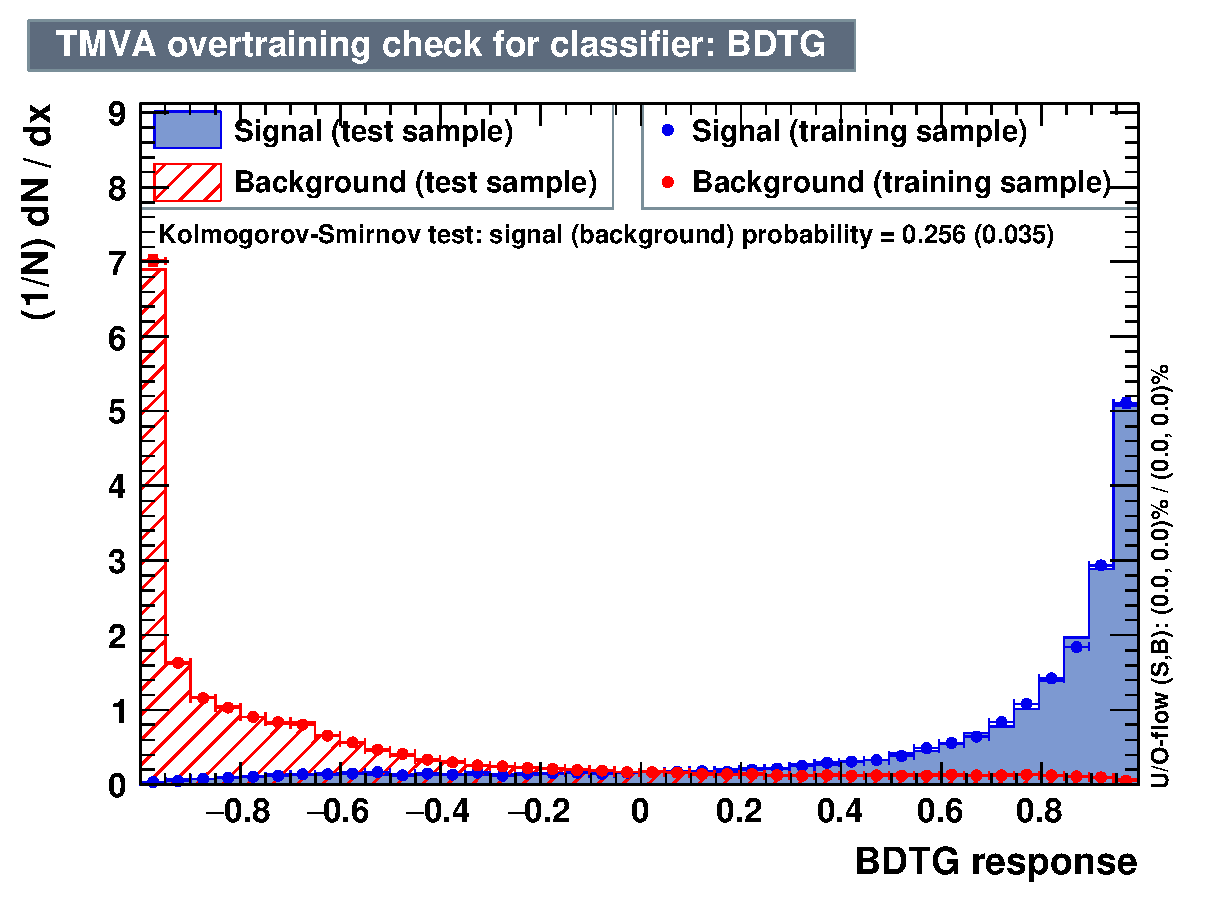
\includegraphics[width=10cm]{NuECCMVAOvertrainBDT.eps}
  \caption[The MVA response when training $\nu_e$ (signal) against $\nu_{\mu}$ and $\nu_{\tau}$ (background).]{The MVA response when training $\nu_e$ (signal) against $\nu_{\mu}$ and $\nu_{\tau}$ (background) using the variables described in Section~\ref{sec:FDMVAVariables}.}
  \label{fig:MVAResponse}
\end{figure}

The efficiency and purity distributions for the selection, over a number of observable kinematic variables, are shown in Figure~\ref{fig:EffPurNoSelection} for all events before applying the selection and in Figure~\ref{fig:EffPurSelection} following the implementation of the MVA cut.

\begin{figure}
  \centering
  \begin{subfigure}[t]{0.48\linewidth}
    \centering
    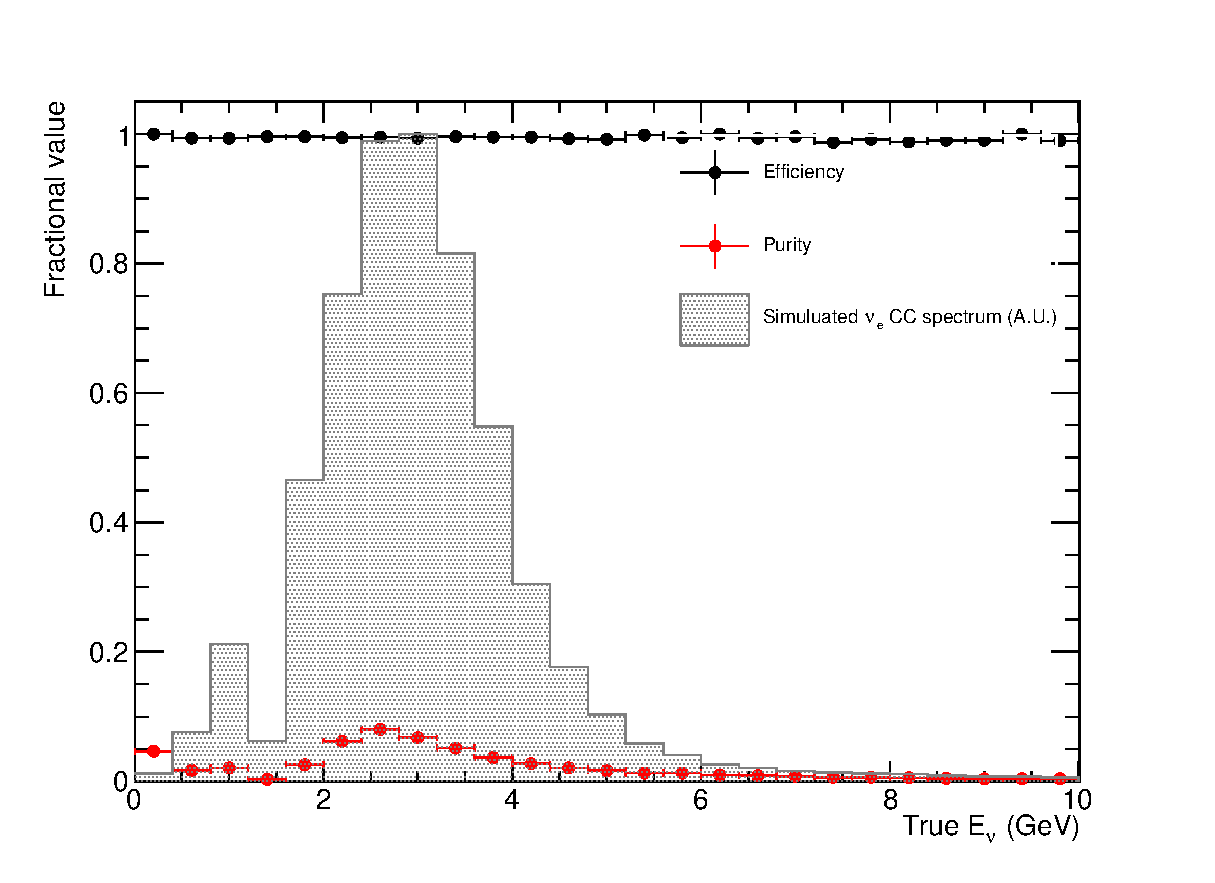
\includegraphics[width=0.98\textwidth]{ENuNoSelection.eps}
    \caption{$E_{\nu}$}
    \label{fig:ENuNoSelection}
  \end{subfigure}
  \hfill
  \begin{subfigure}[t]{0.48\linewidth}
    \centering
    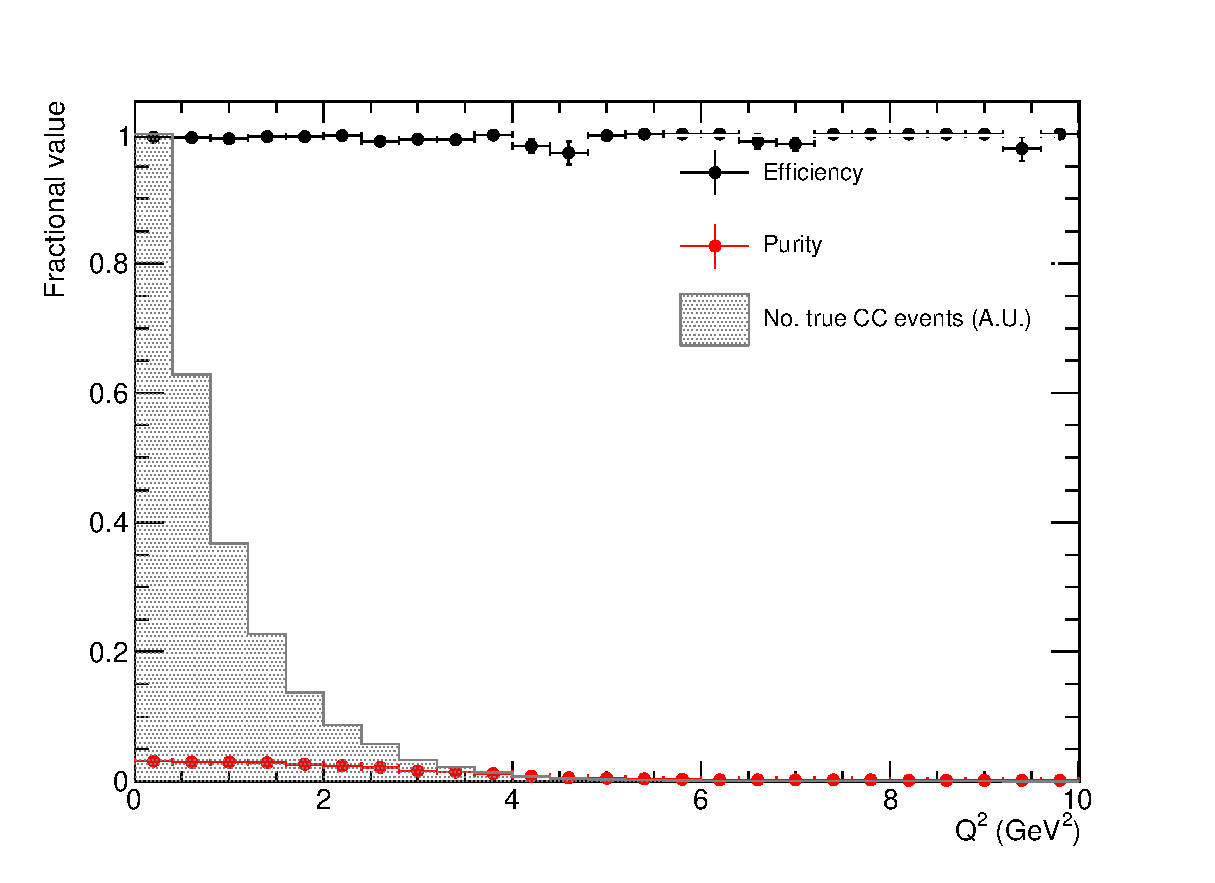
\includegraphics[width=0.98\textwidth]{Q2NoSelection.eps}
    \caption{$Q^2$}
    \label{fig:Q2NoSelection}
  \end{subfigure}
  \vfill
  \begin{subfigure}[t]{0.48\linewidth}
    \centering
    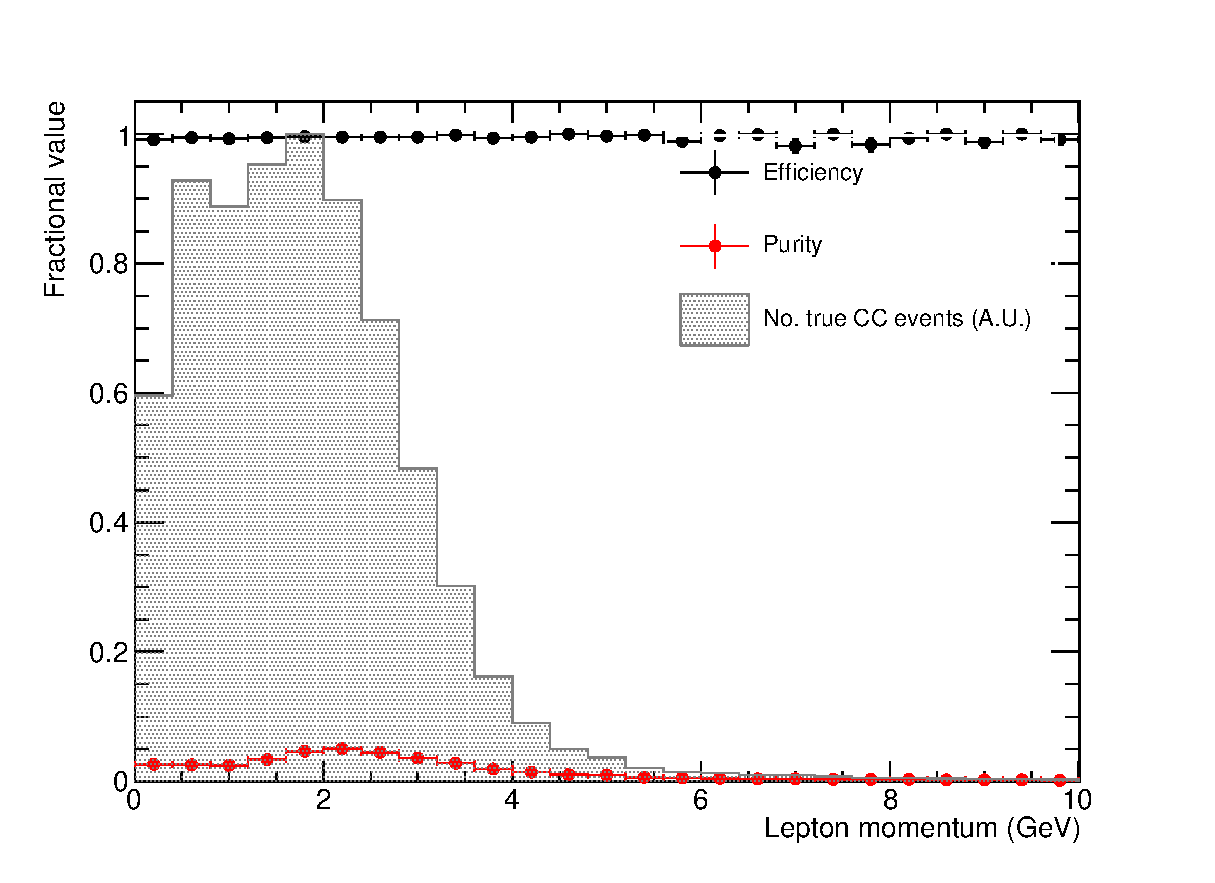
\includegraphics[width=0.98\textwidth]{LeptonMomentumNoSelection.eps}
    \caption{Lepton momentum}
    \label{fig:LeptonMomentumNoSelection}
  \end{subfigure}
  \hfill
  \begin{subfigure}[t]{0.48\linewidth}
    \centering
    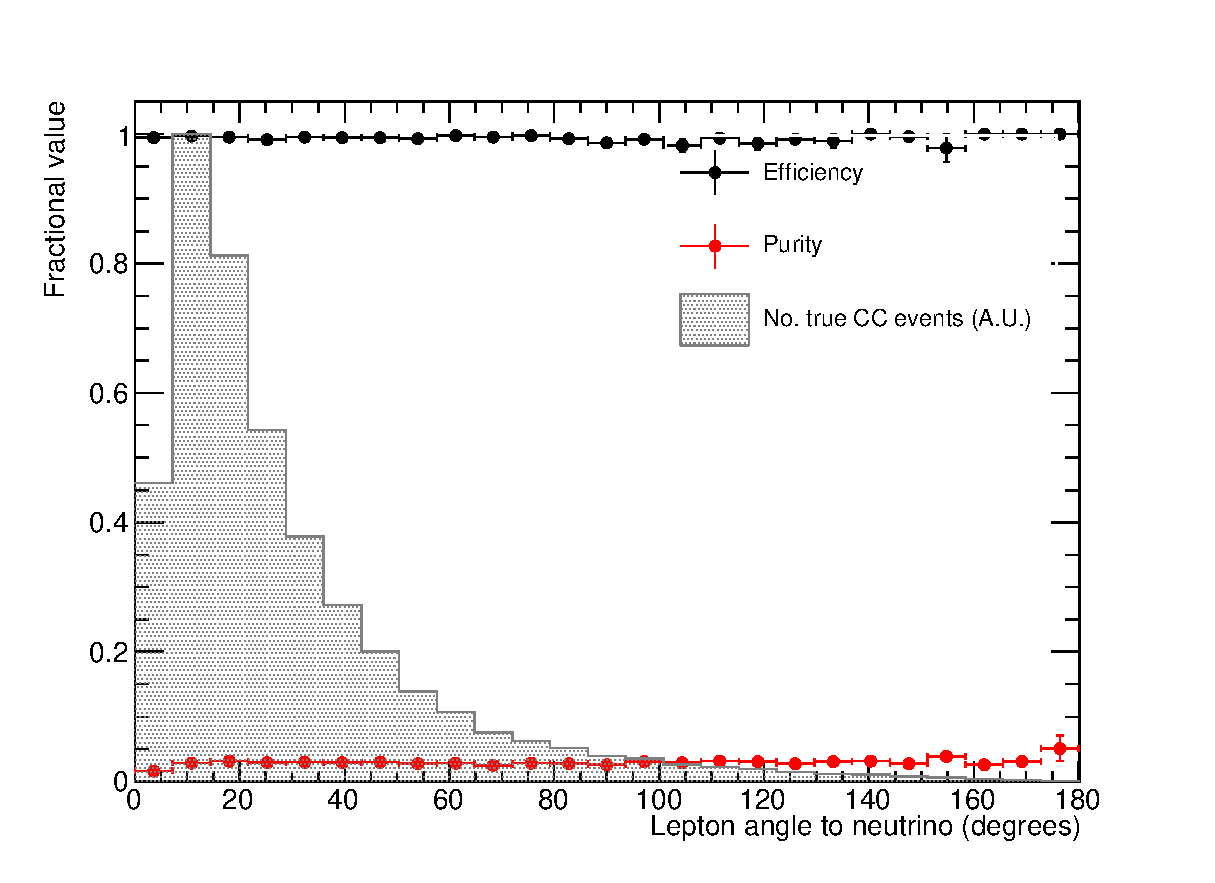
\includegraphics[width=0.98\textwidth]{LeptonAngleNoSelection.eps}
    \caption{Lepton angle}
    \label{fig:LeptonAngleNoSelection}
  \end{subfigure}
  \caption[The efficiency and purity of the $\nu_e$CC MVA-based selection as a function of a number of kinematic variables, before applying the selection.]{The efficiency and purity of the $\nu_e$CC MVA-based selection as a function of a number of kinematic variables, before applying the selection.  The variables are the true neutrino energy (Figure~\ref{fig:ENuNoSelection}), the true momentum transfer, $Q^2$ (Figure~\ref{fig:Q2NoSelection}), the electron momentum (Figure~\ref{fig:LeptonMomentumNoSelection}) and the angle the electron makes to the neutrino beam (Figure~\ref{fig:LeptonAngleNoSelection}).  The plots are filled for each event with reconstruction within the fiducial volume.  Given the relaxed restrictions on this region currently, described in Section~\ref{sec:FDCutFV}, these distributions may be expected to change significantly when using a more realistic FV.}
  \label{fig:EffPurNoSelection}
\end{figure}

\begin{figure}
  \centering
  \begin{subfigure}[t]{0.48\linewidth}
    \centering
    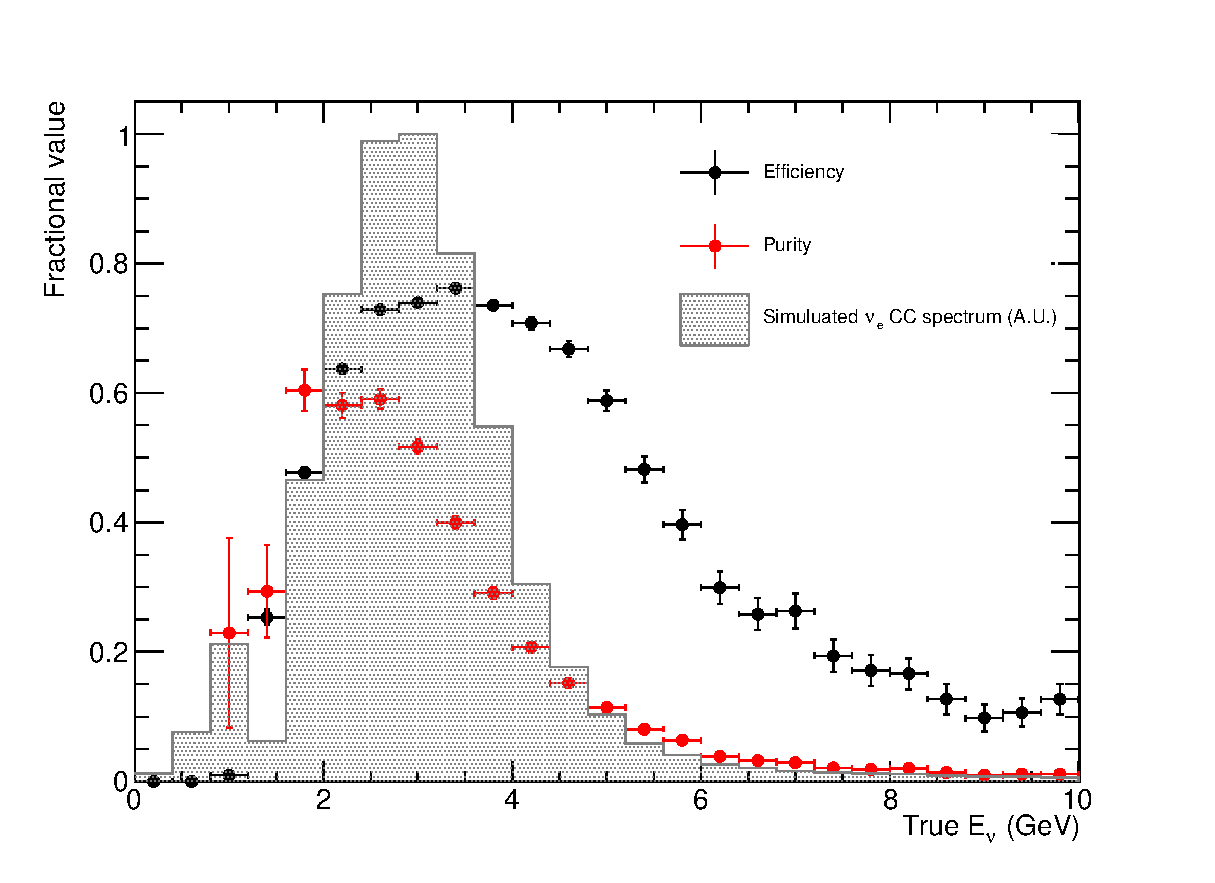
\includegraphics[width=0.98\textwidth]{ENuSelection.eps}
    \caption{$E_{\nu}$}
    \label{fig:ENuSelection}
  \end{subfigure}
  \hfill
  \begin{subfigure}[t]{0.48\linewidth}
    \centering
    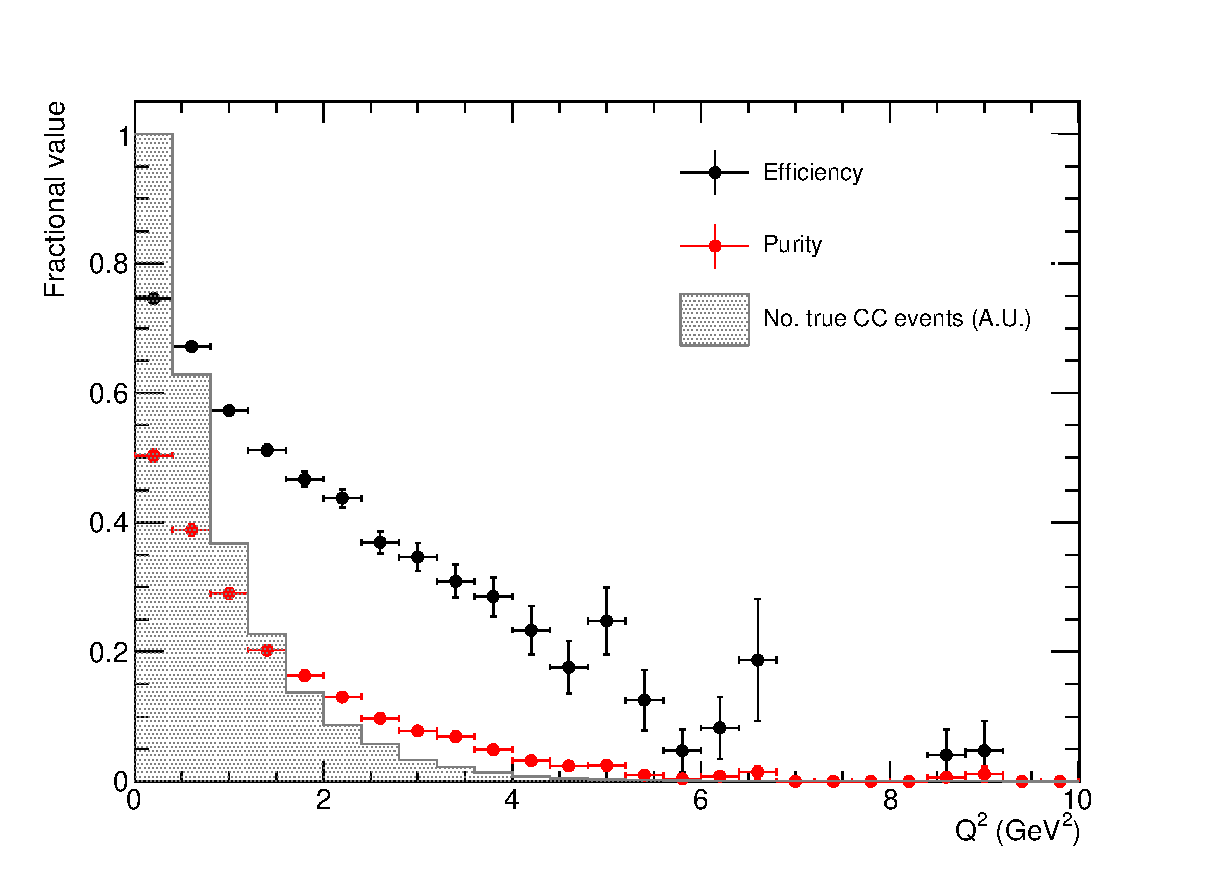
\includegraphics[width=0.98\textwidth]{Q2Selection.eps}
    \caption{$Q^2$}
    \label{fig:Q2Selection}
  \end{subfigure}
  \vfill
  \begin{subfigure}[t]{0.48\linewidth}
    \centering
    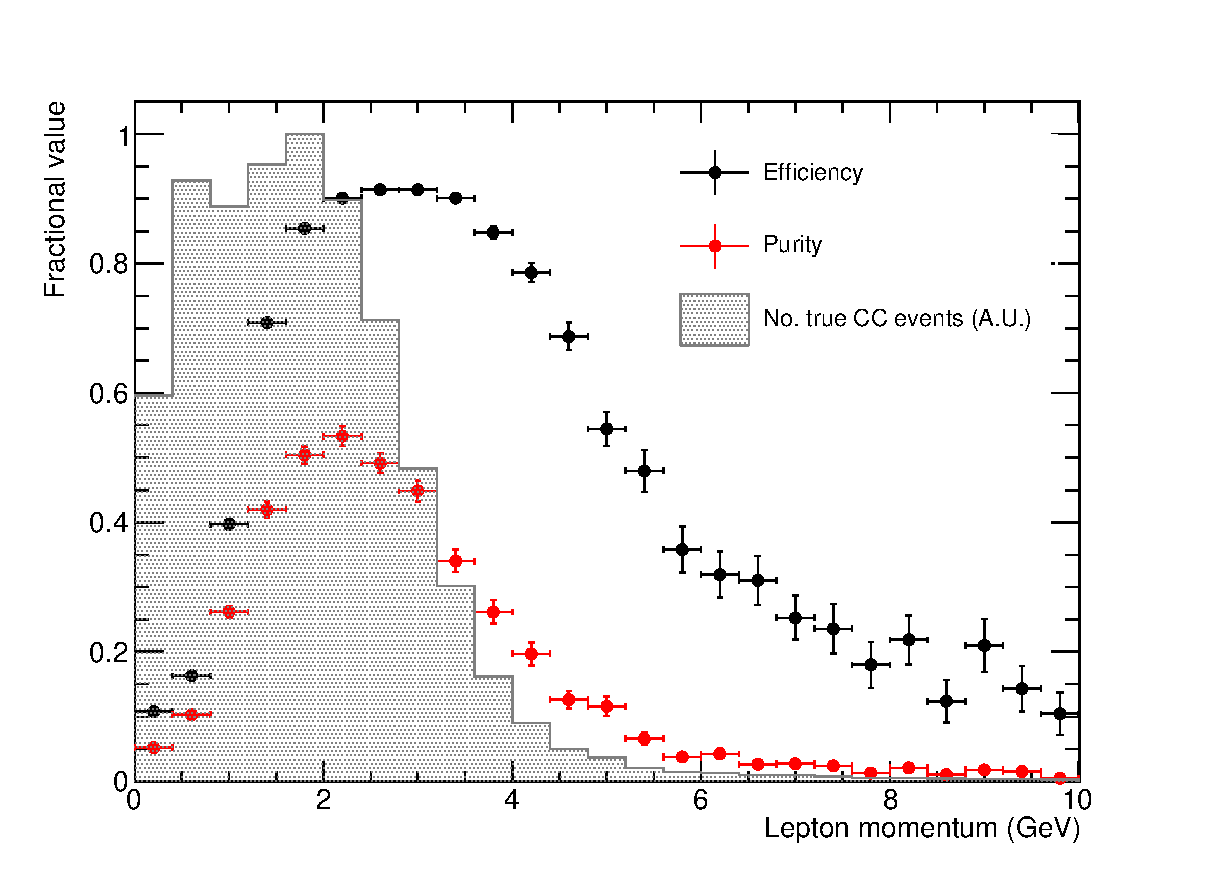
\includegraphics[width=0.98\textwidth]{LeptonMomentumSelection.eps}
    \caption{Lepton momentum}
    \label{fig:LeptonMomentumSelection}
  \end{subfigure}
  \hfill
  \begin{subfigure}[t]{0.48\linewidth}
    \centering
    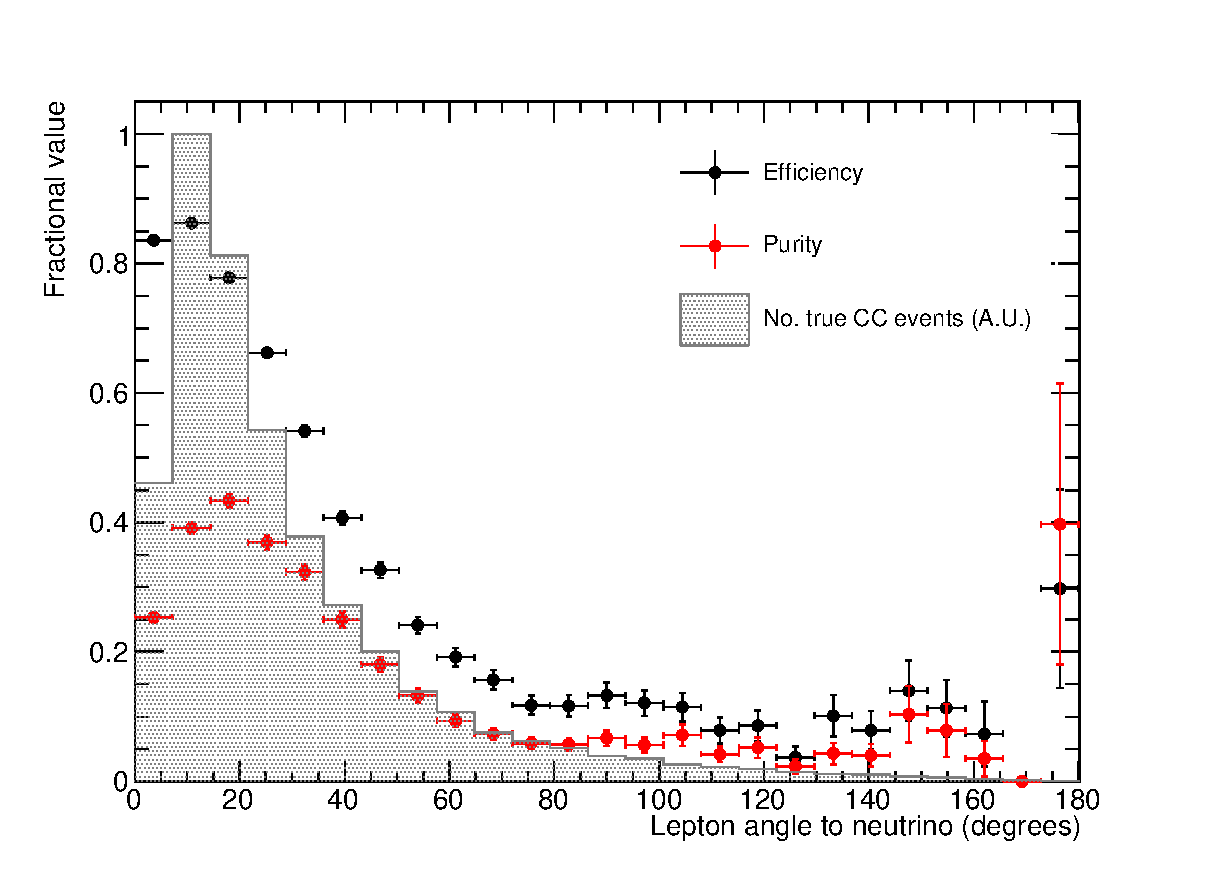
\includegraphics[width=0.98\textwidth]{LeptonAngleSelection.eps}
    \caption{Lepton angle}
    \label{fig:LeptonAngleSelection}
  \end{subfigure}
  \caption[The efficiency and purity of the $\nu_e$CC MVA-based selection as a function of a number of kinematic variables, after applying the selection.]{The efficiency and purity of the $\nu_e$CC MVA-based selection as a function of a number of kinematic variables, after applying the selection.  The variables are the true neutrino energy (Figure~\ref{fig:ENuSelection}), the true momentum transfer, $Q^2$ (Figure~\ref{fig:Q2Selection}), the electron momentum (Figure~\ref{fig:LeptonMomentumSelection}) and the angle the electron makes to the neutrino beam (Figure~\ref{fig:LeptonAngleSelection}).  The plots are filled for each event which passes the cut (MVA response $>0.81$).}
  \label{fig:EffPurSelection}
\end{figure}

Overall, the selection is shown to have an efficiency of 52\% and a purity of 63\%.  The biases in the selection around the distribution of events are evident from the plots in Figure~\ref{fig:EffPurSelection} and have not yet been fully understood.  This potentially may not be a significant issue but does require further comprehension and is being addressed using the selection discussed in Section~\ref{sec:FDCut}, where the effects observed in the assessment of the MVA-based analysis were not present and instead the performance was more directly correlated with the kinematic variables (shown in Figure~\ref{fig:EffPurCutSelection}).  Given that the PID MVA utilised in the cut-based selection employs many of the same particle-level variables as in this present implementation, it appears a more natural approach to the problem.  By incorporating the event-level information to the selection on top of this basis, a more thorough evaluation of the interactions is possible.  As already discussed, this work is ongoing.

%----------------------------------------------------------------------------------------------------------------------------------------------------------------------------
\section{Outlook for Future Selections}\label{sec:FDOutlook}

The analysis presented in Section~\ref{sec:FDMVA} is a promising first step towards the eventual DUNE $\nu_e$CC selection.  There are still many improvements to be made in general but specifically in the event reconstruction, as discussed in Section~\ref{sec:ReconstructionPerformance}, and in the current implementation of the selection.  In addition to the MVA and Pandora cut-based studies, a significant effort in utilising the CVN machine learning techniques, which have been successfully demonstrated in the NO$\nu$A experiment \cite{Aurisano2016}, for this purpose is underway.

The current rate of development within the LArSoft and DUNE collaborations is significant and progress over the next decade will facilitate a high-precision study of the electron neutrino appearance channel in the DUNE far detector.  This is of critical importance to the success of the DUNE project and, considering the efforts presented in this thesis in both the reconstruction (Chapter~\ref{chap:LArTPCReconstruction}) and the selection (Chapter~\ref{chap:FDAnalysis}), there can be much confidence in the future of the analysis and the potential discovery power of the experiment.
